\documentclass[border=0.2cm]{standalone}

\usepackage{tikz}
\usetikzlibrary{automata, arrows.meta, positioning}

\begin{document}

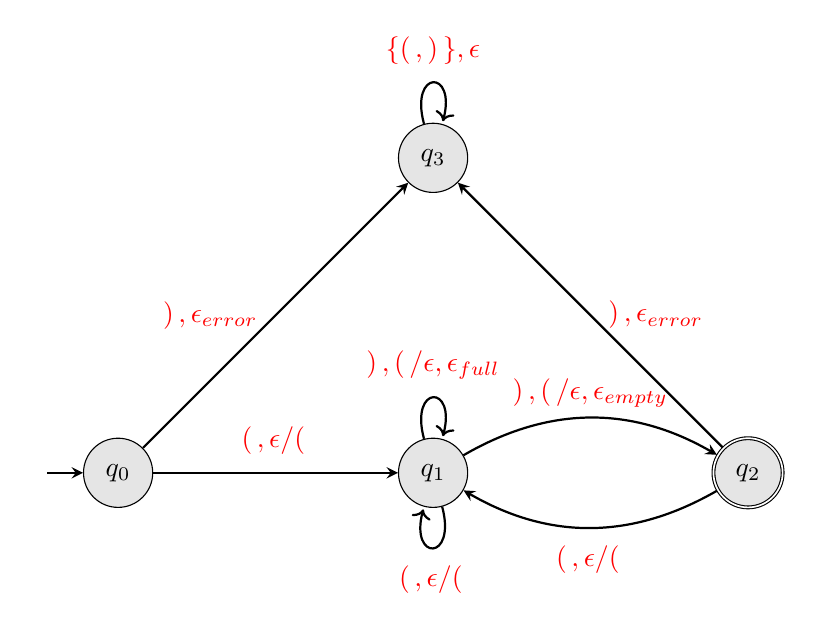
\begin{tikzpicture} [node distance = 4cm, on grid, auto,every state/.style = {fill = gray!20},
every initial by arrow/.style = {font = \large, text = red, thick,-stealth}]

\node (q0) [state, initial, initial text = {}] {$q_0$};
\node (q1) [state, right = of q0] {$q_1$};
\node (q2) [state, accepting, right = of q1] {$q_2$};
\node (q3) [state, above = of q1] {$q_3$};

\path [-stealth,thick,text=red]
	(q0) edge  node [above=0.1cm] {$(\,,\epsilon / (\, $} (q1)
    (q0) edge  node [left=0.1cm] {$)\,,\epsilon_{error} $} (q3)
    (q1) edge [bend left] node[above] {$)\,, (\, / \epsilon, \epsilon_{empty} $} (q2)
    (q1) edge [loop below] node [below=0.1cm] {$(\,,\epsilon /(\,$ } (q1)
    (q1) edge [loop above] node [above=0.1cm] {$)\,, (\, / \epsilon, \epsilon_{full}$ } (q1)
	(q2) edge [bend left] node[below=0.1cm] {$(\,,\epsilon / (\, $} (q1)
    (q2) edge  node [right=0.1cm] {$)\,,\epsilon_{error}$} (q3)
    (q3) edge [loop above] node [above=0.1cm] {$\{(\,,)\,\}, \epsilon$} (q3);
\end{tikzpicture}

\end{document}
